% !TeX root = ../main.tex

%%% Tables %%%

\begin{table}[h]
\centering
\caption{Accuracies and run times for all models. All reported values are averages, and $\pm$ refers to the standard deviation. The run times heavily depend upon the optimization method.}
\begin{tabular}{ccccccc}
Model       & \multicolumn{1}{c}{Training Time (Minutes)} & \multicolumn{1}{c}{Dive Accuracy} & \multicolumn{1}{c}{Subdive Accuracy}  \\ \hline
CarHMM-DFT  & $61.68 \pm 10.21$                            & -------------                     & $1.00 \pm 0.00$                       \\ 
HHMM-DFT    & $139.76 \pm 28.93$                           & $0.94 \pm 0.03$                   & $1.00 \pm 0.00$                       \\
CarHHMM     & $257.58 \pm 81.64$                           & $0.87 \pm 0.11$                   & $0.89 \pm 0.01$                       \\
CarHHMM-DFT & $150.18 \pm 36.94$                           & $0.94 \pm 0.02$                   & $1.00 \pm 0.00$                       \\
\end{tabular}
\label{table:accuracy}
\end{table}

\begin{table}[ht]
    \centering
    \caption{Estimates and standard errors of emission parameters for killer whale data.}
    \scalebox{0.8}{
\begin{tabular}{ccccc}
\multirow{2}{*}{Feature}                                                       & \multirow{2}{*}{Dive / Subdive Type} & \multicolumn{3}{c}{Parameter Estimate}              \\
                                                                               &                                      & $\hat \mu$      & $\hat \sigma$   & $\hat \phi$     \\ \hline
\multirow{2}{*}{Dive Duration $(s)$ - $Y$}                                     & 1                                    & $25.69 \pm 0.60$ & $9.57 \pm 0.51$ & ---             \\
                                                                               & 2                                    & $104.60 \pm 9.39$ & $64.68 \pm 7.47$ & ---             \\ \hline
\multirow{3}{*}{x-acceleration $(m/s^2)$ - $\left(\mathbf{Z}^{*(1)}\right)_x$} & 1                                    & $0.02 \pm 0.04$ & $0.03 \pm 0.00$ & $0.98 \pm 0.01$ \\
                                                                               & 2                                    & $0.24 \pm 0.01$ & $0.08 \pm 0.00$ & $0.89 \pm 0.01$ \\
                                                                               & 3                                    & $0.22 \pm 0.03$ & $0.27 \pm 0.01$ & $0.63 \pm 0.03$ \\ \hline
\multirow{3}{*}{y-acceleration $(m/s^2)$ - $\left(\mathbf{Z}^{*(1)}\right)_y$} & 1                                    & $0.47 \pm 0.05$ & $0.04 \pm 0.00$ & $0.98 \pm 0.01$ \\
                                                                               & 2                                    & $0.44 \pm 0.01$ & $0.08 \pm 0.00$ & $0.89 \pm 0.01$ \\
                                                                               & 3                                    & $0.38 \pm 0.03$ & $0.32 \pm 0.01$ & $0.63 \pm 0.03$ \\ \hline
\multirow{3}{*}{z-acceleration $(m/s^2)$ - $\left(\mathbf{Z}^{*(1)}\right)_z$} & 1                                    & $-0.68 \pm 0.06$ & $0.05 \pm 0.00$ & $0.98 \pm 0.01$ \\
                                                                               & 2                                    & $-0.59 \pm 0.02$ & $0.10 \pm 0.00$ & $0.89 \pm 0.01$ \\
                                                                               & 3                                    & $-0.37 \pm 0.03$ & $0.32 \pm 0.01$ & $0.63 \pm 0.03$ \\ \hline
\multirow{3}{*}{Fourier sum - $Z^{*(2)}$}                                      & 1                                    & $23.34 \pm 0.28$ & $12.95 \pm 0.27$ & ---             \\
                                                                               & 2                                    & $301.19 \pm 3.24$ & $330.05 \pm 4.17$ & ---             \\
                                                                               & 3                                    & $10204.01 \pm 211.24$ & $15299.07 \pm 352.67$ & ---             \\ \hline
\end{tabular}
    }
    \label{table:emis_dists}
\end{table}

%%% model definitions %%%

\begin{figure}[ht]
    \begin{subfigure}{\textwidth}
      \centering
      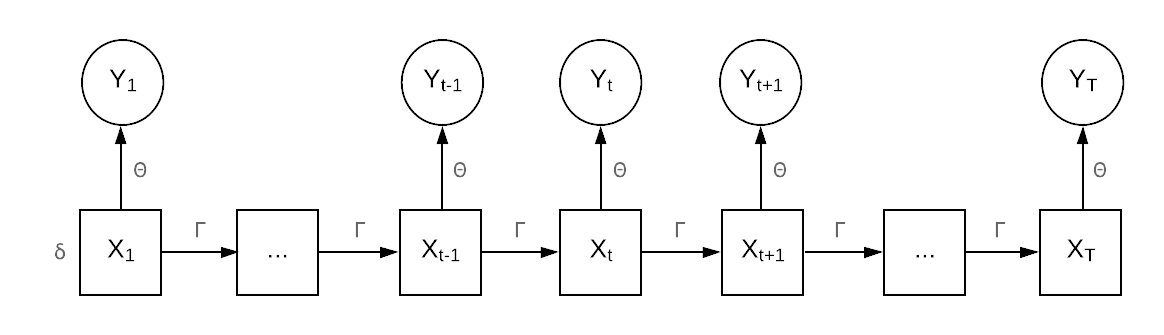
\includegraphics[width=4in]{../Plots/HMM.png}  
      \caption{Hidden Markov Model (\textbf{HMM})}
      \label{fig:HMM}
    \end{subfigure}
    %
    \newline
    %
    \begin{subfigure}{\textwidth}
      \centering
      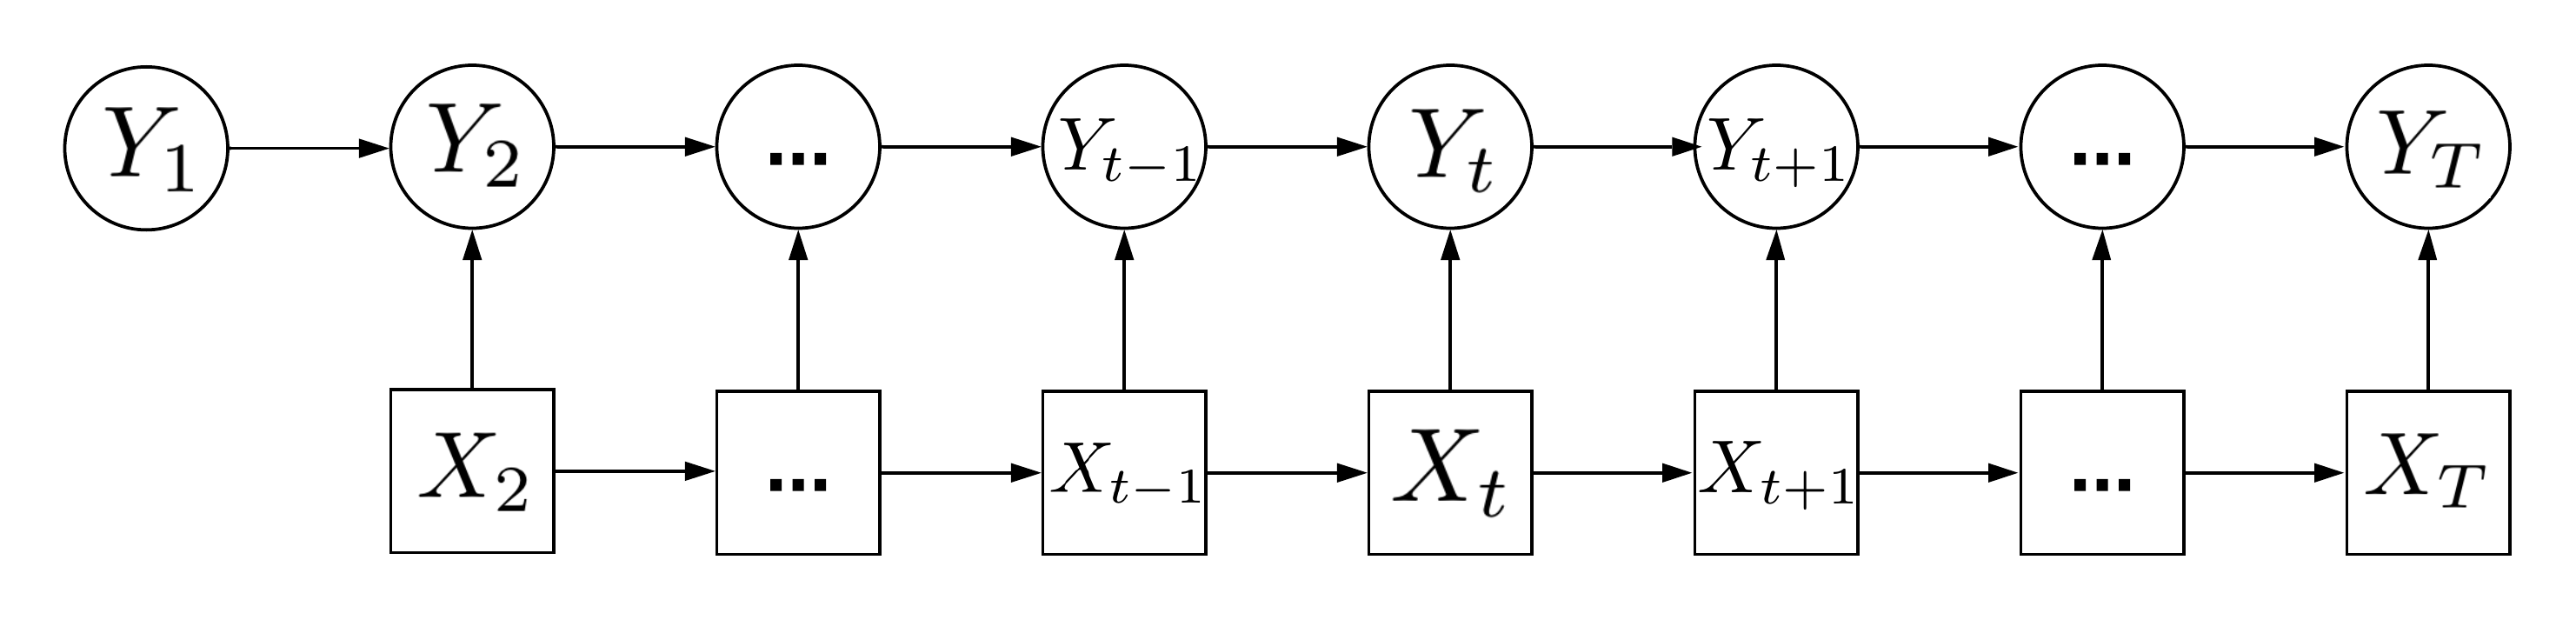
\includegraphics[width=4in]{../Plots/CarHMM.png}  
      \caption{Conditionally Auto-regressive HMM (\textbf{CarHMM})}
      \label{fig:CarHMM}
    \end{subfigure}
    %
    \newline
    %
    \begin{subfigure}{\textwidth}
      \centering
      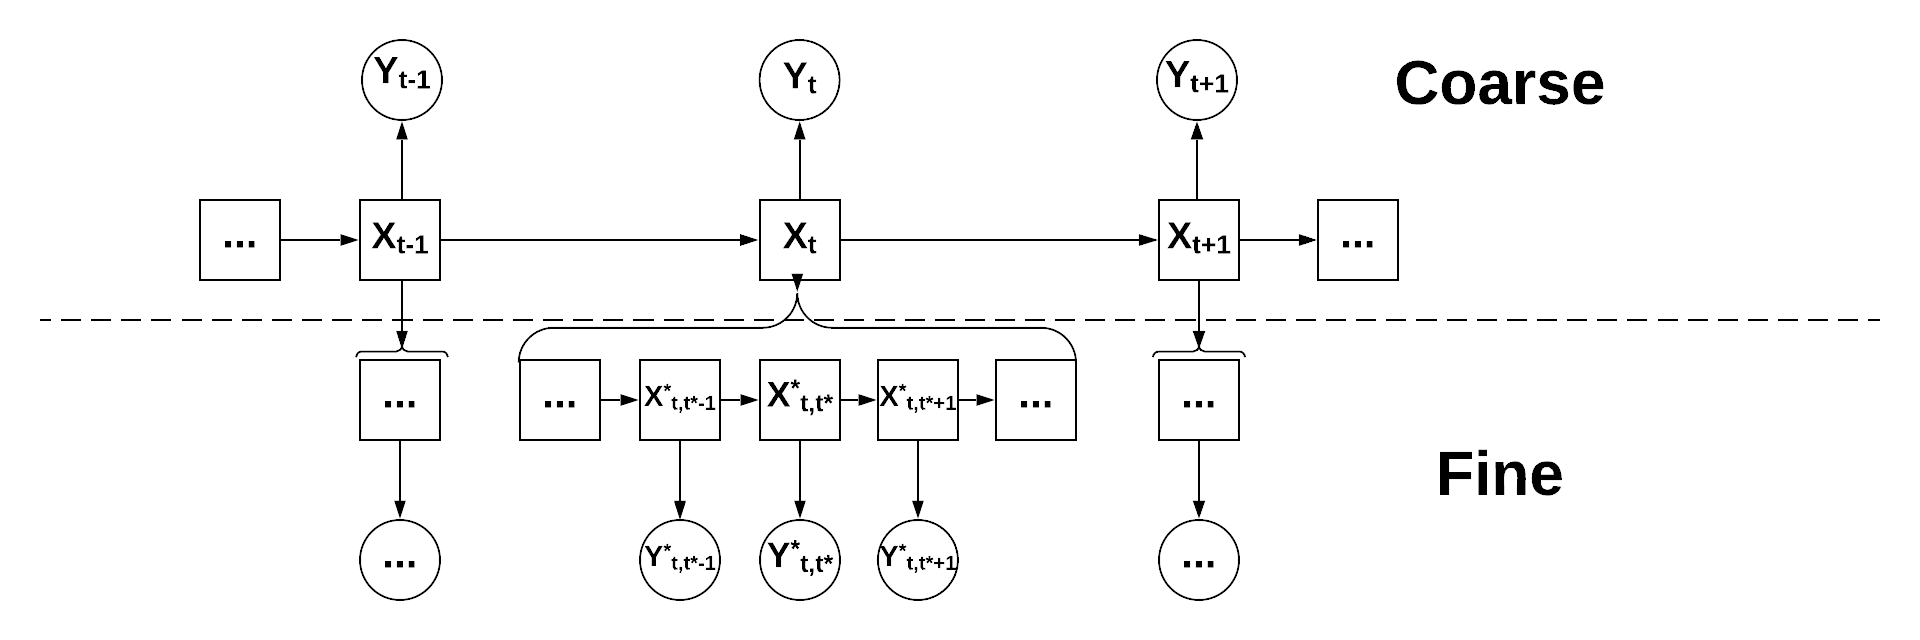
\includegraphics[width=4in]{../Plots/HHMM.png}  
      \caption{Hierarchical HMM (\textbf{HHMM})}
      \label{fig:HHMM}
    \end{subfigure}
    %
    \newline
    %
    \begin{subfigure}{\textwidth}
      \centering
      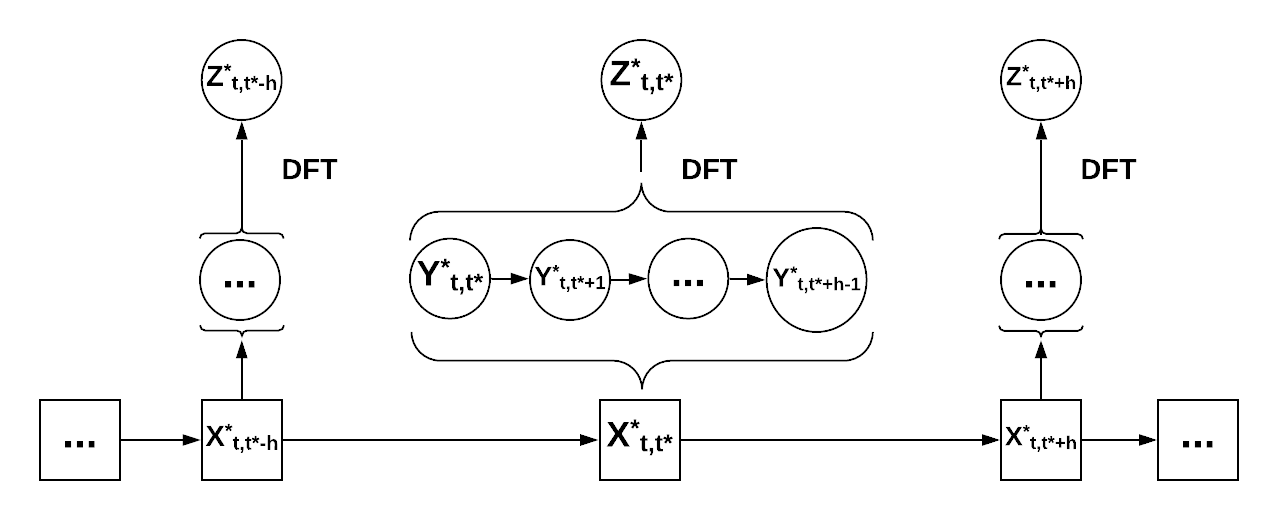
\includegraphics[width=4in]{../Plots/HMM-DFT.png}  
      \caption{HMM with Discrete Fourier Transform (\textbf{HMM-DFT})}
      \label{fig:HMM-DFT}
    \end{subfigure}
    \caption{Graphical representations of HMM models}
    \label{fig:models}
\end{figure}

%%% simulation study %%%

\begin{figure}[ht]
	\centering
	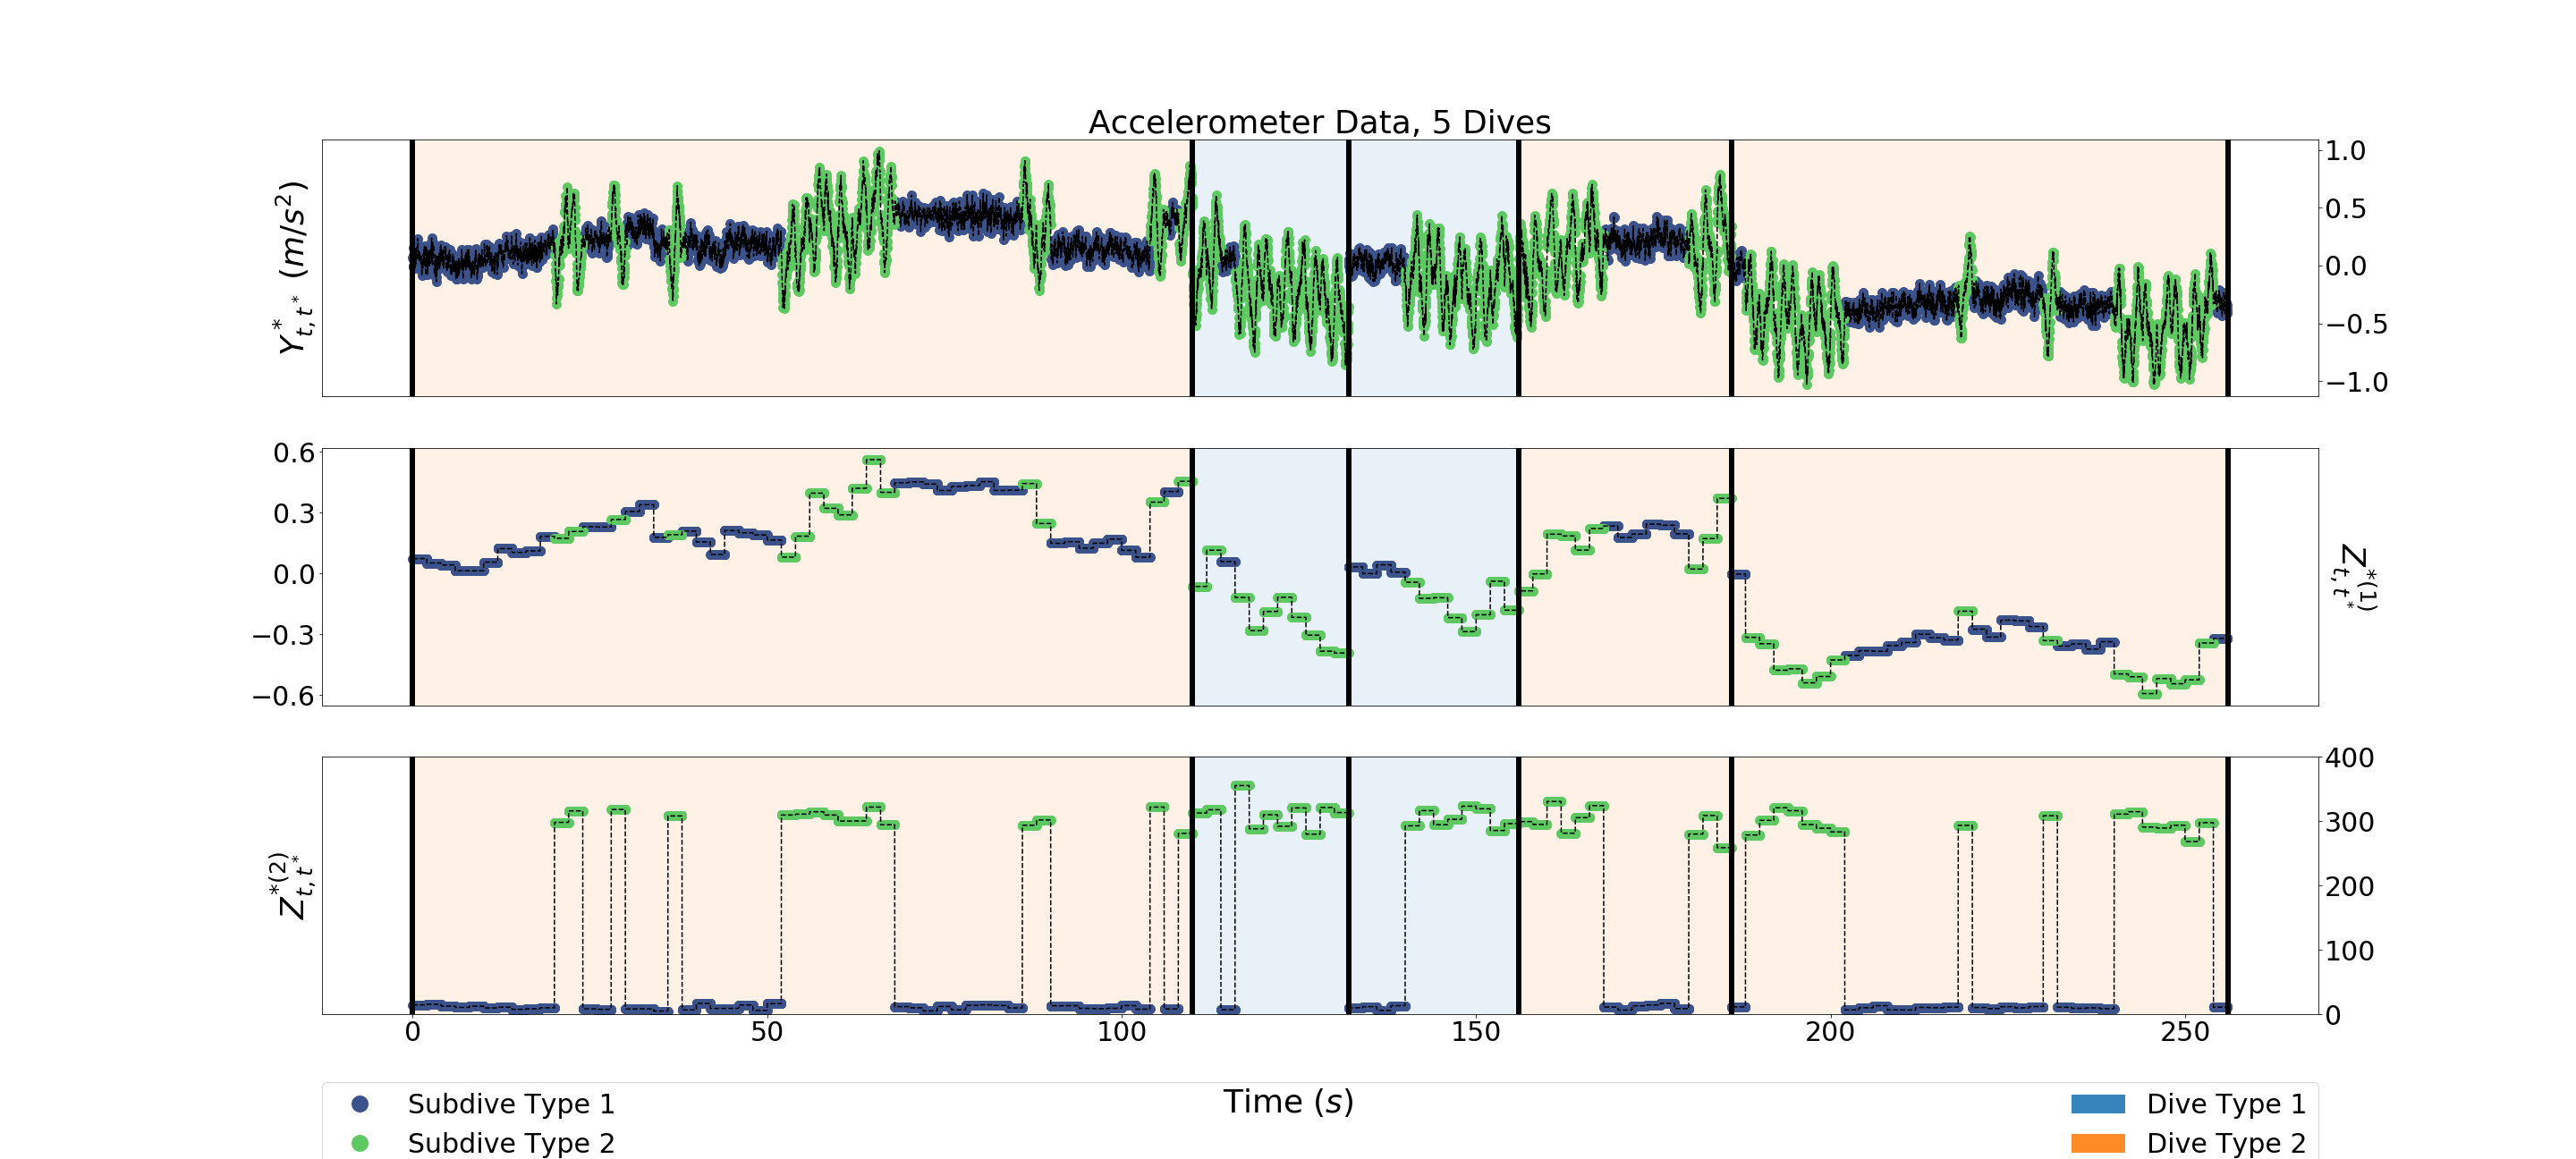
\includegraphics[width=5.5in]{../Plots/sim_data.png}
	\caption{Simulated acceleration data for one dive. The color of the line corresponds to the true fine-scale state of the sub-dive process, while the color of the background corresponds to the true dive type of the simulated whale.}
	\label{fig:sim_data}
\end{figure}

\begin{figure}[ht]
	\centering
	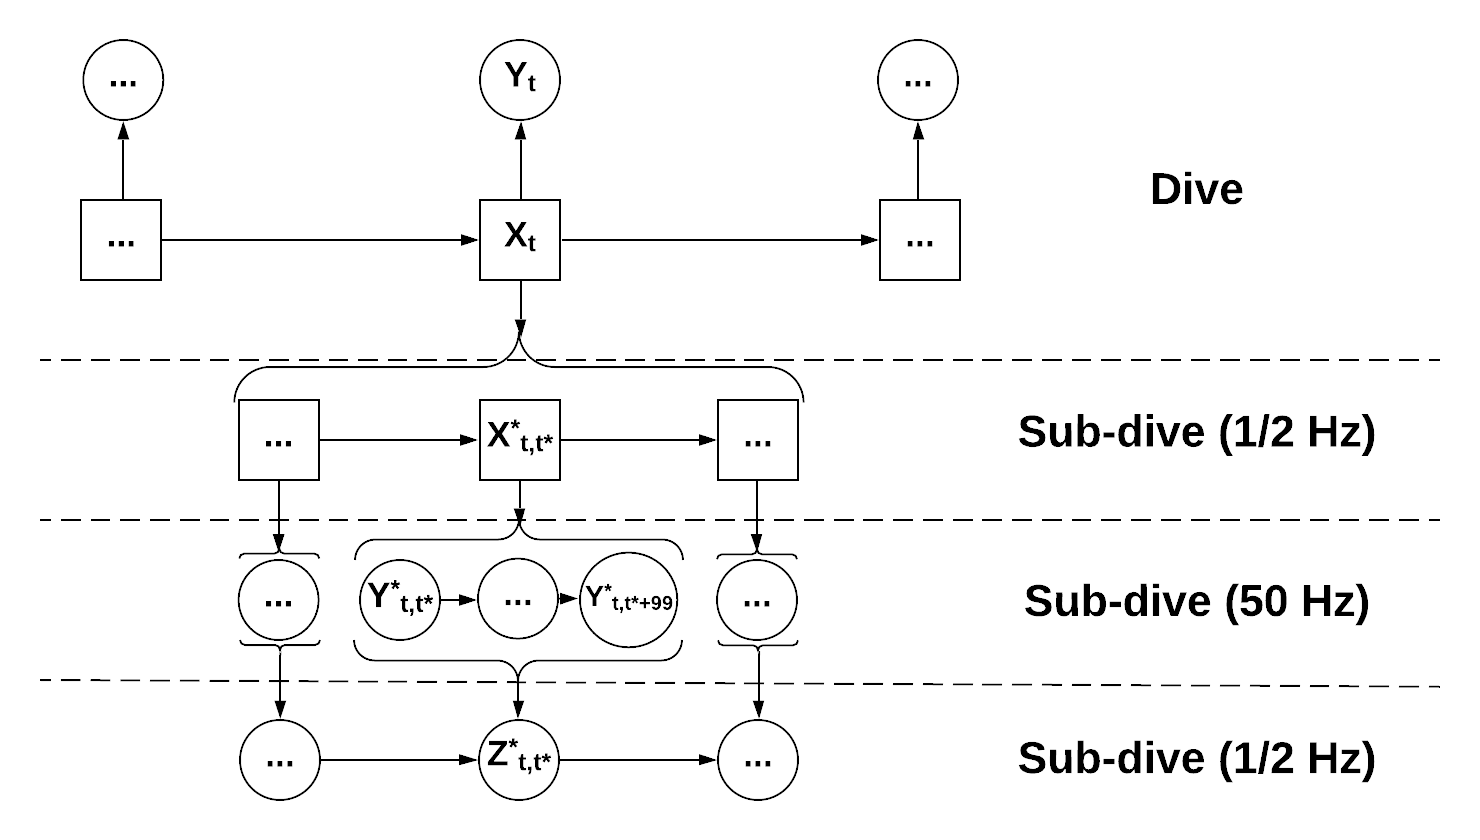
\includegraphics[width=5in]{../Plots/CarHHMM-DFT.png}
	\caption{Graphical representation the model used in the simulation and case study, the \textbf{CarHHMM-DFT}.}
	\label{fig:CarHHMM-DFT}
\end{figure}

\begin{figure}[ht]
    \centering
    \begin{subfigure}[t]{1.0\textwidth}
        \centering
        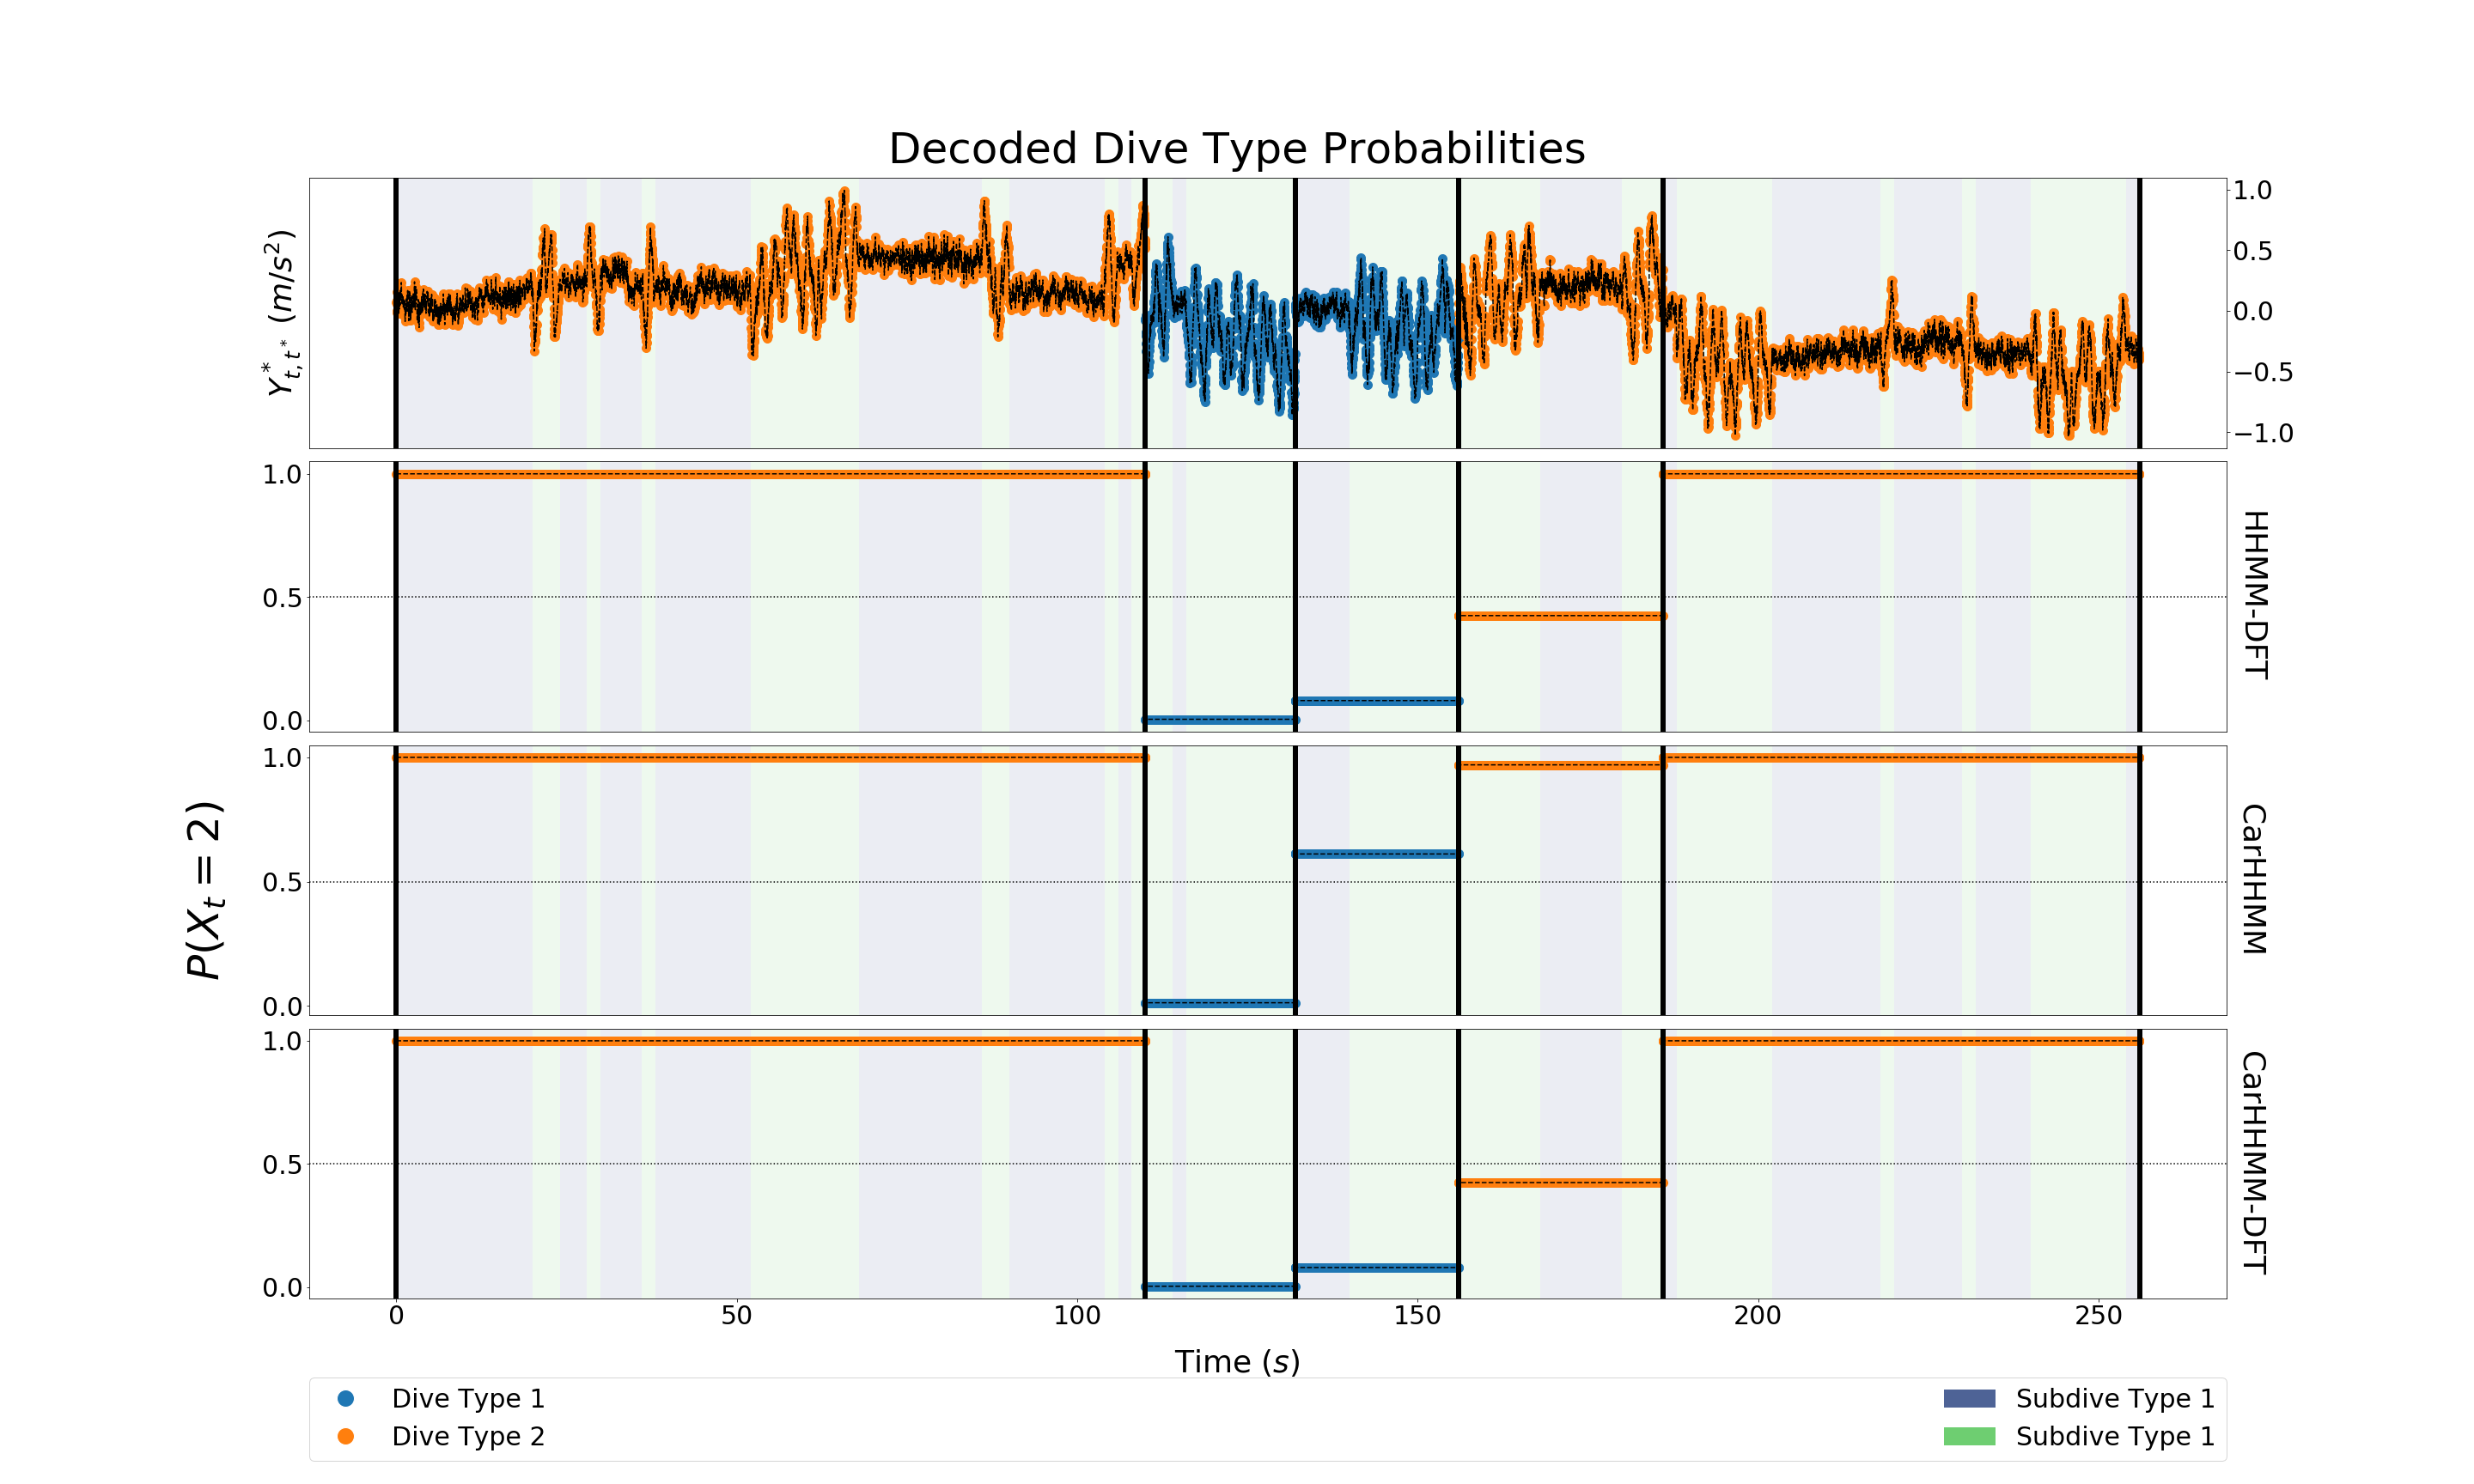
\includegraphics[width=3.5in]{../Plots/Posterior_Coarse_States.png}
        \caption{Coarse-scale hidden process}
    \end{subfigure}
    %
    \begin{subfigure}[t]{1.0\textwidth}
        \centering
        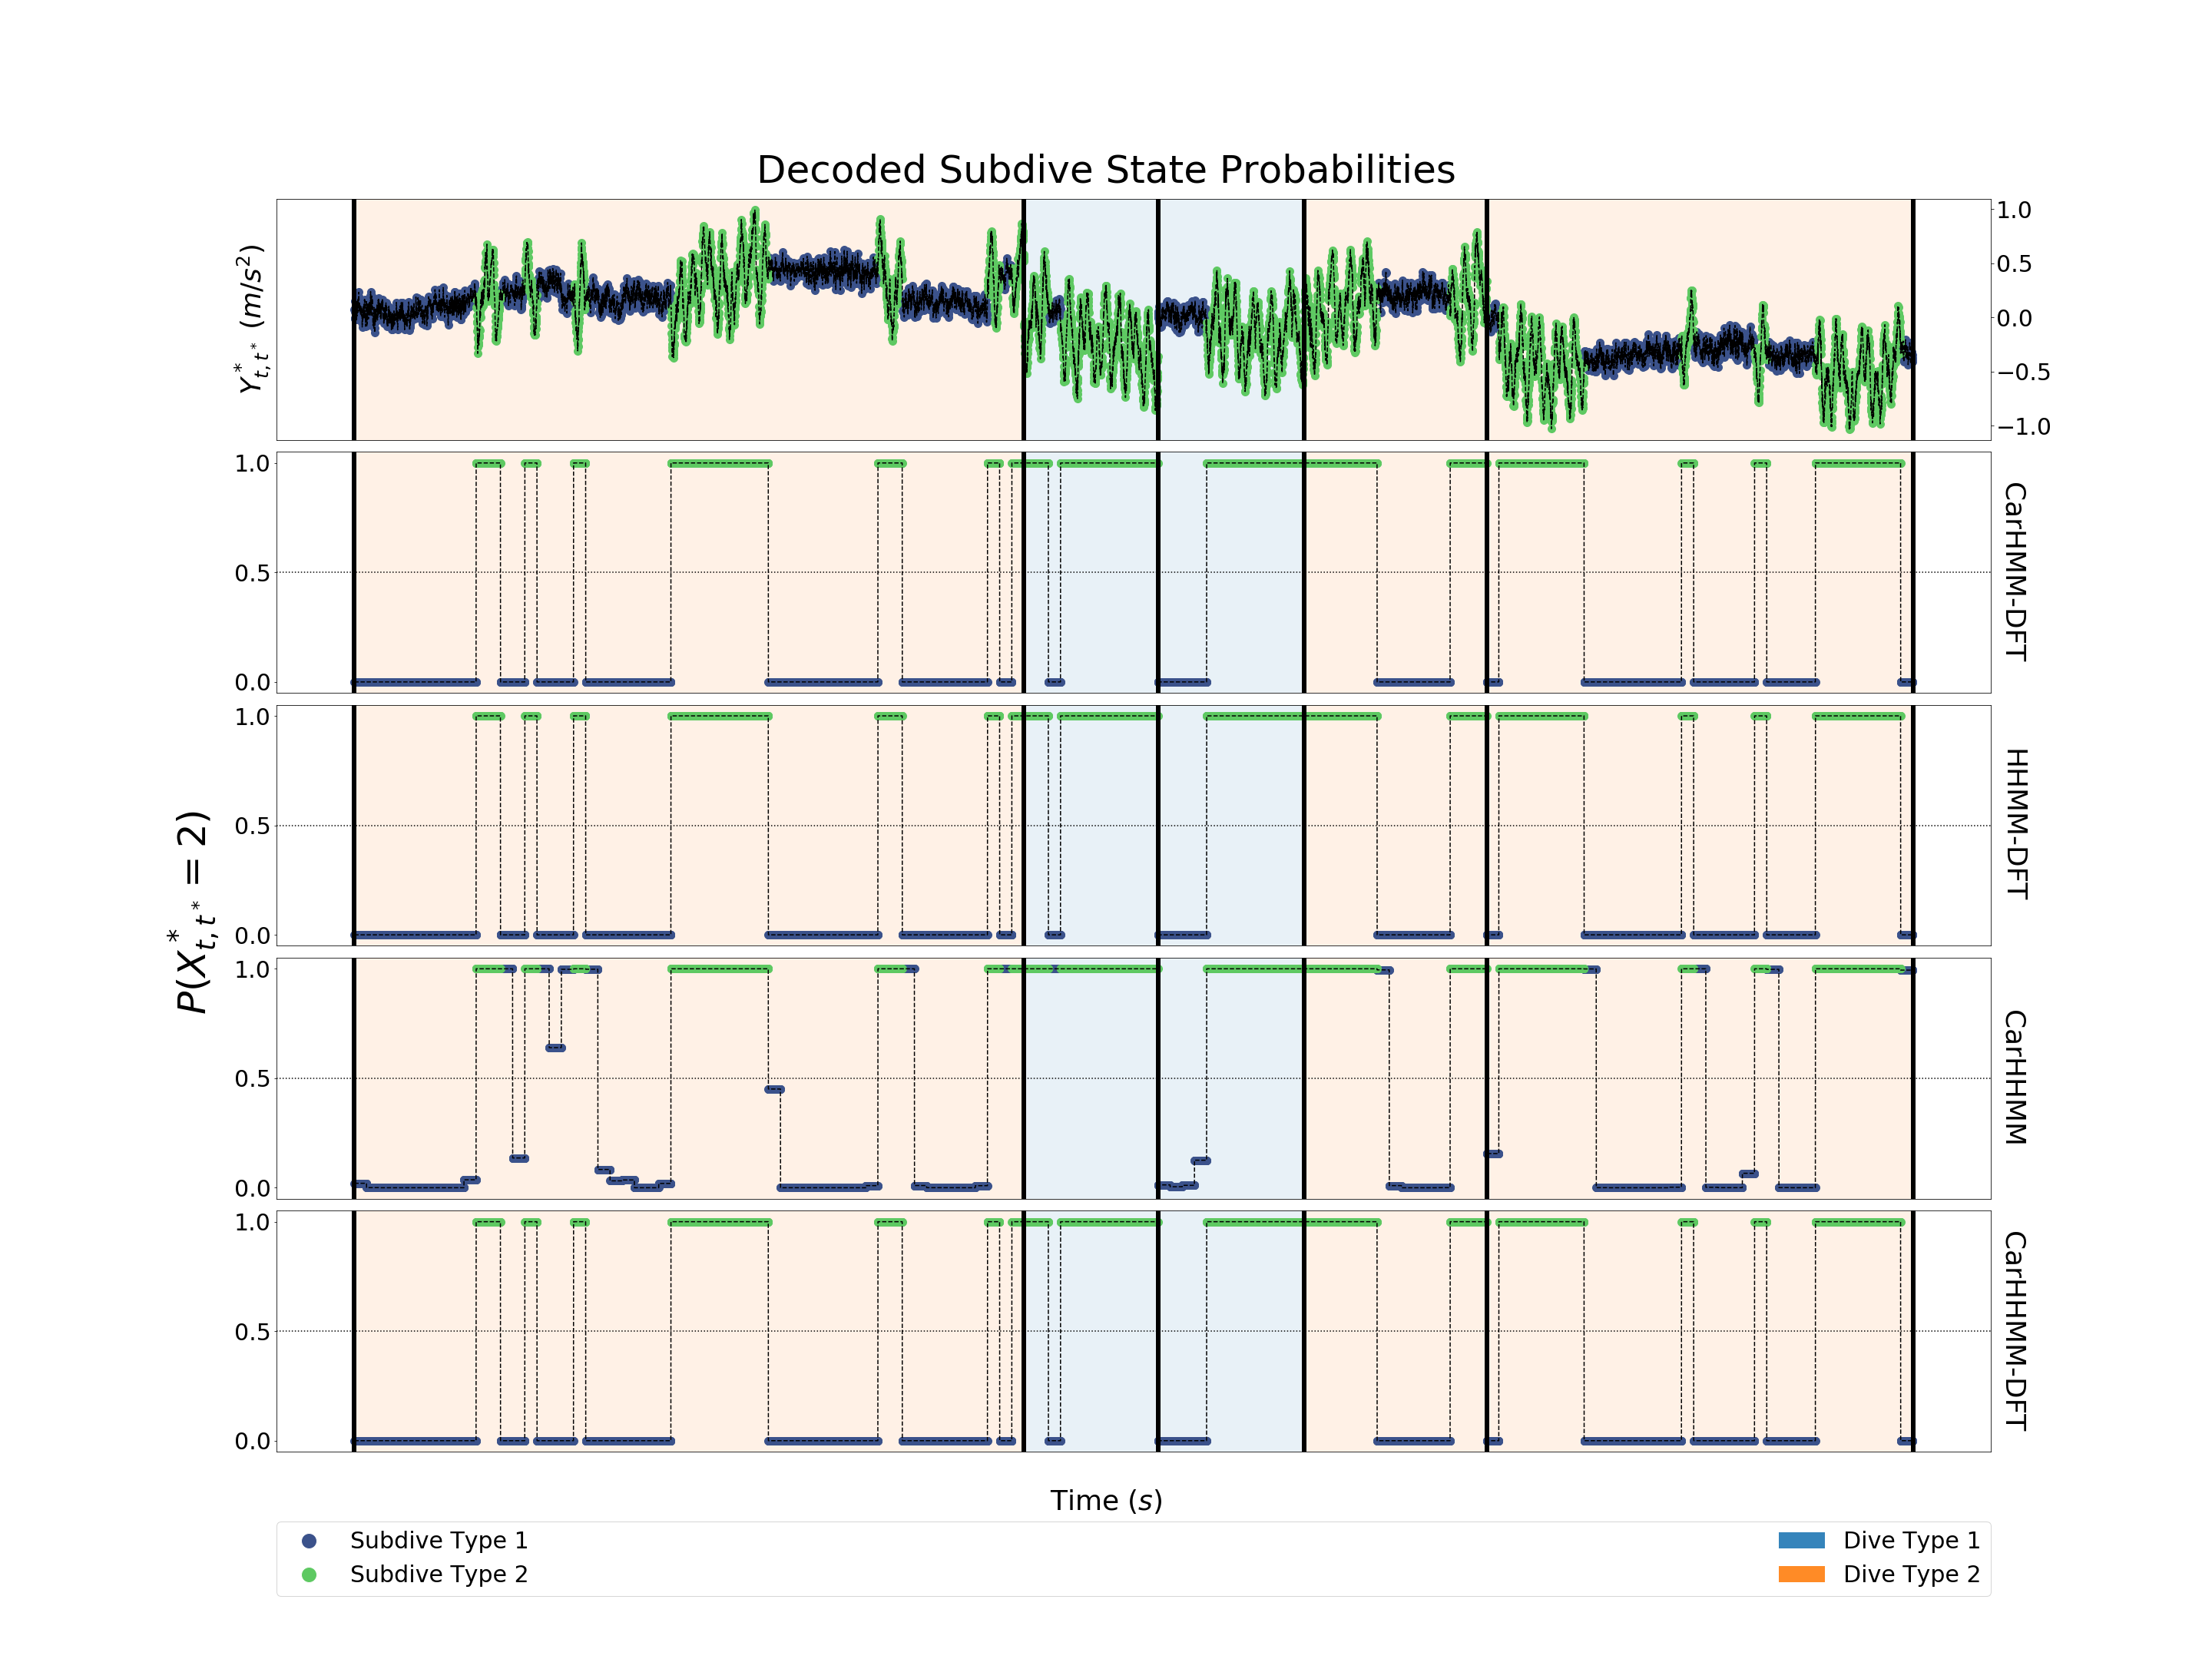
\includegraphics[width=3.5in]{../Plots/Posterior_Fine_States.png}
        \caption{Fine-scale hidden process}
    \end{subfigure}
	\caption{Decoded state probabilities of each model for 5 dives of one simulated data set. The colors correspond to the true behavioral state.}
	\label{fig:acc}
\end{figure}

%%% Case Study %%%

\begin{figure}[ht]
	\centering
	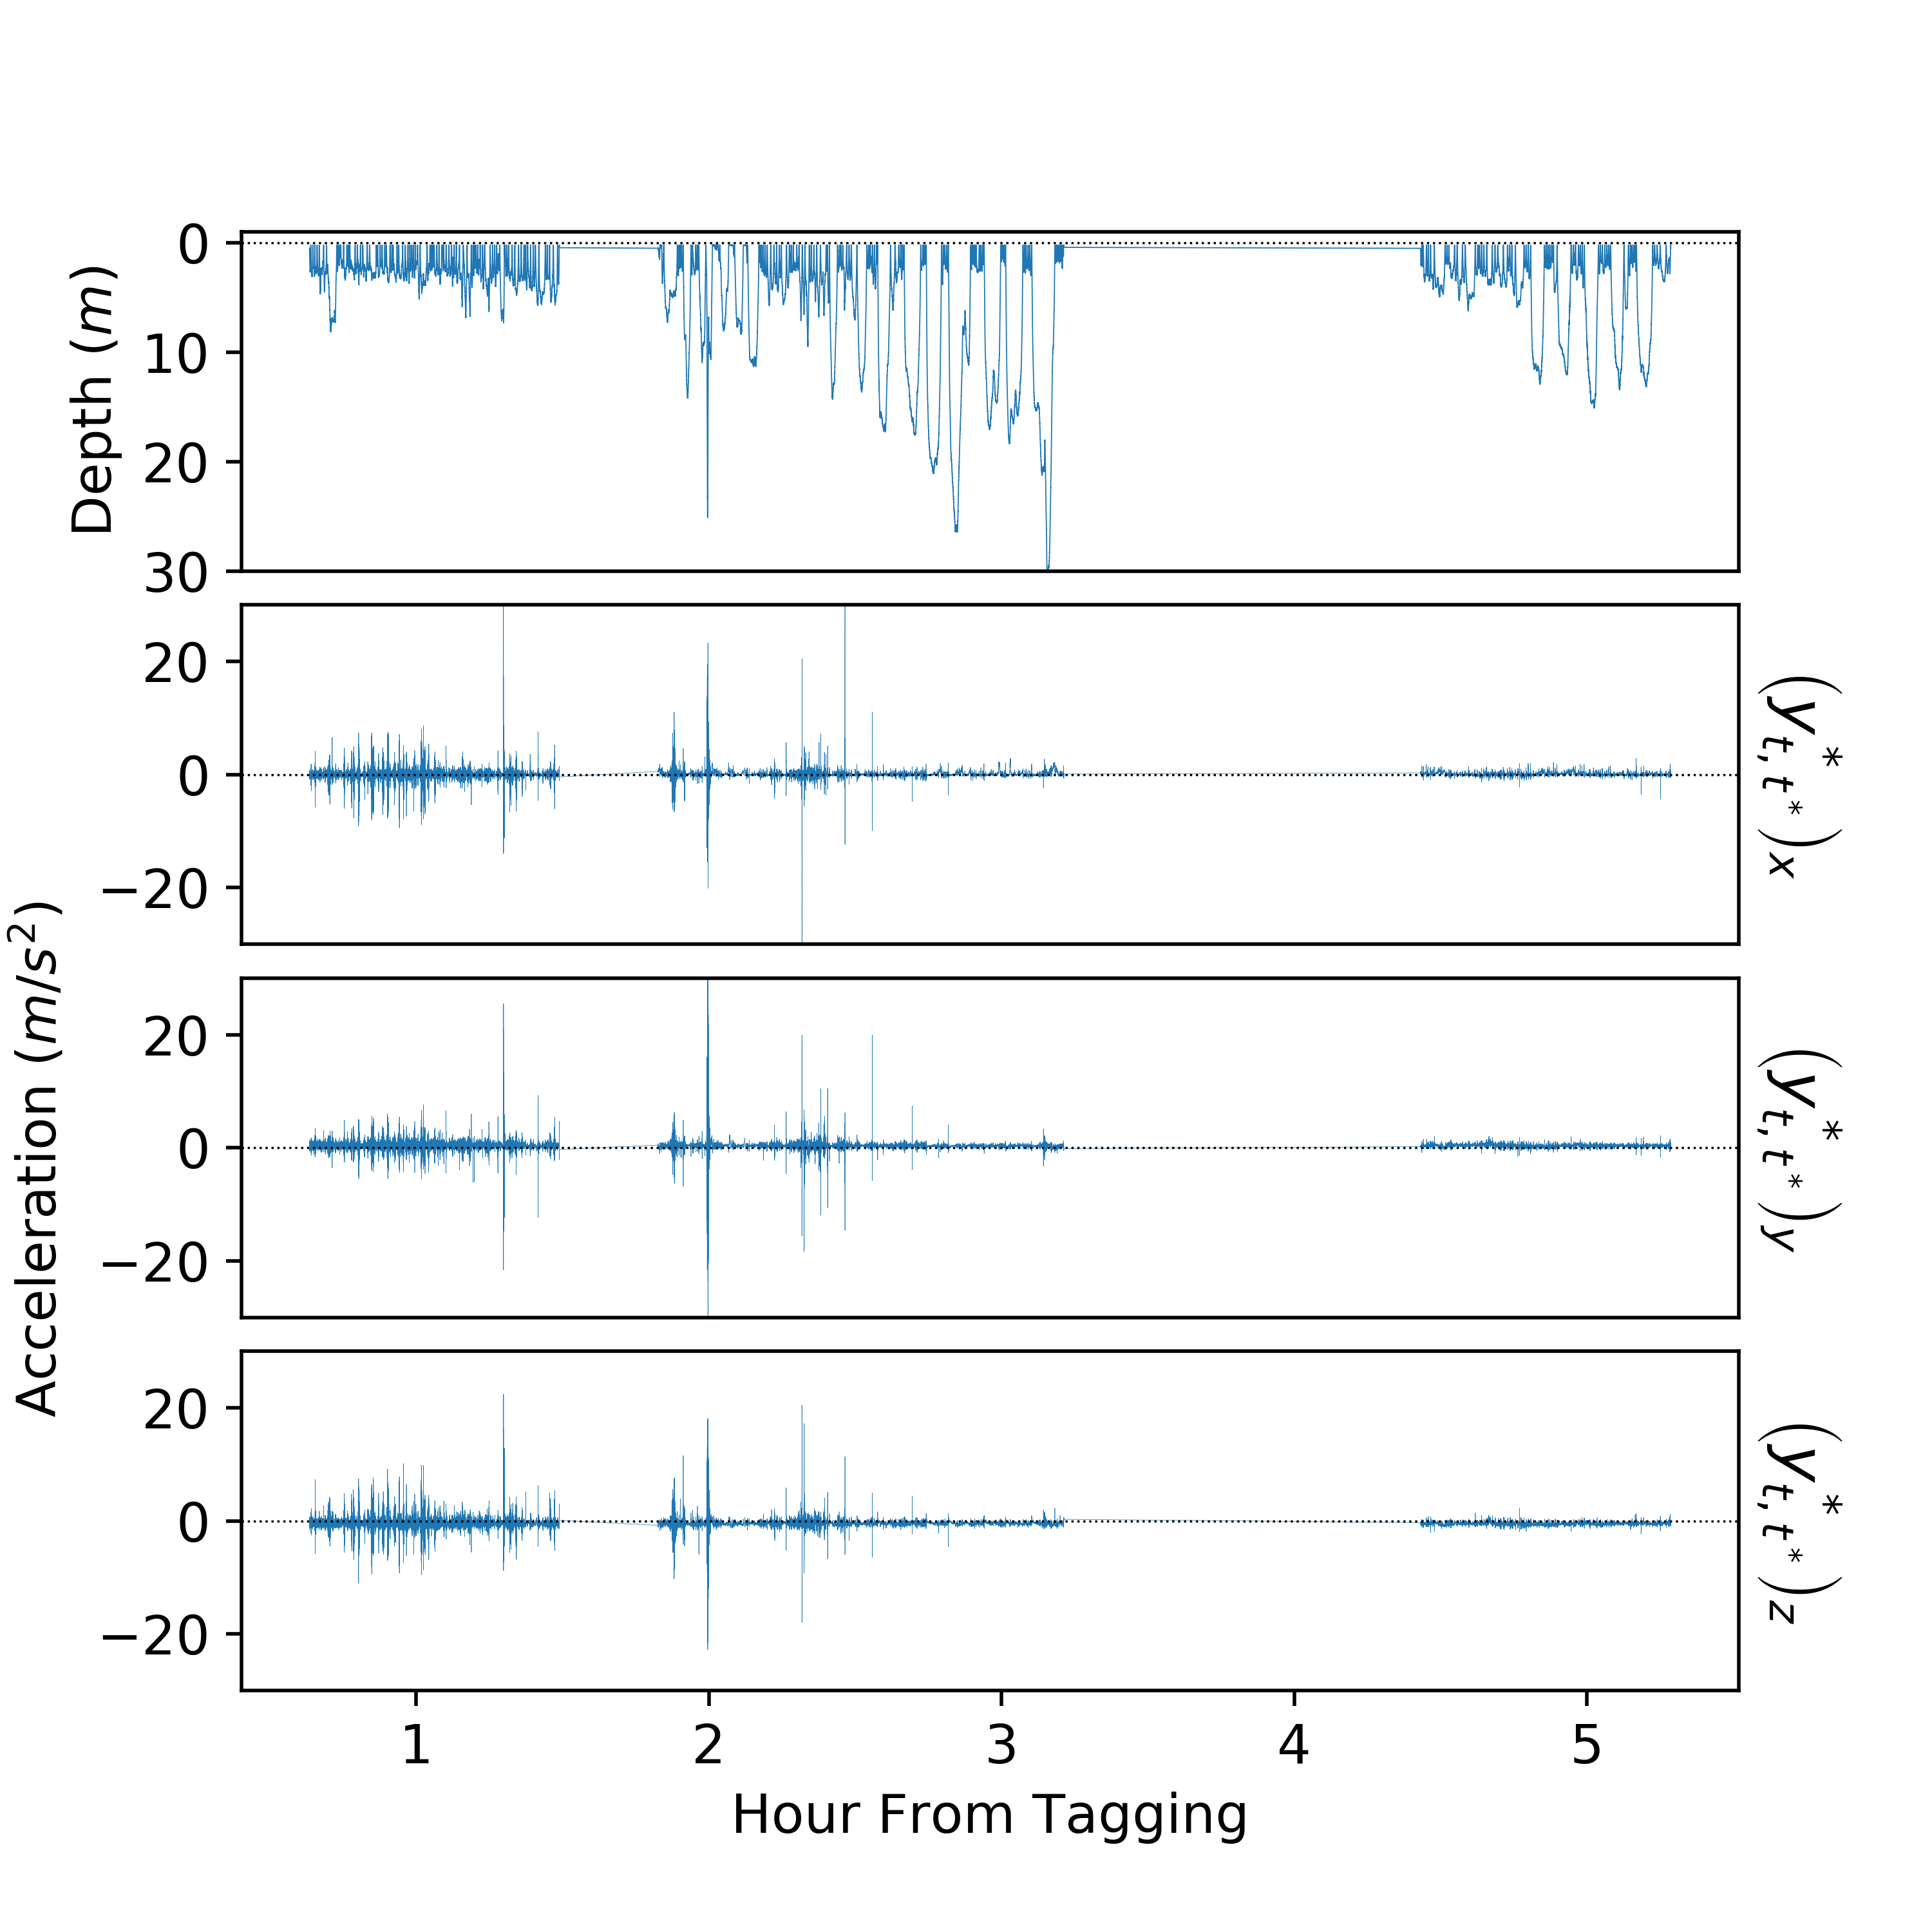
\includegraphics[width=5in]{../Plots/raw_data.png}
	\caption{Dive depth (top panel) and acceleration (bottom three panels) as functions of time, from the killer whale data set}
	\label{fig:data}
\end{figure}

\begin{figure}[ht]
	\centering
	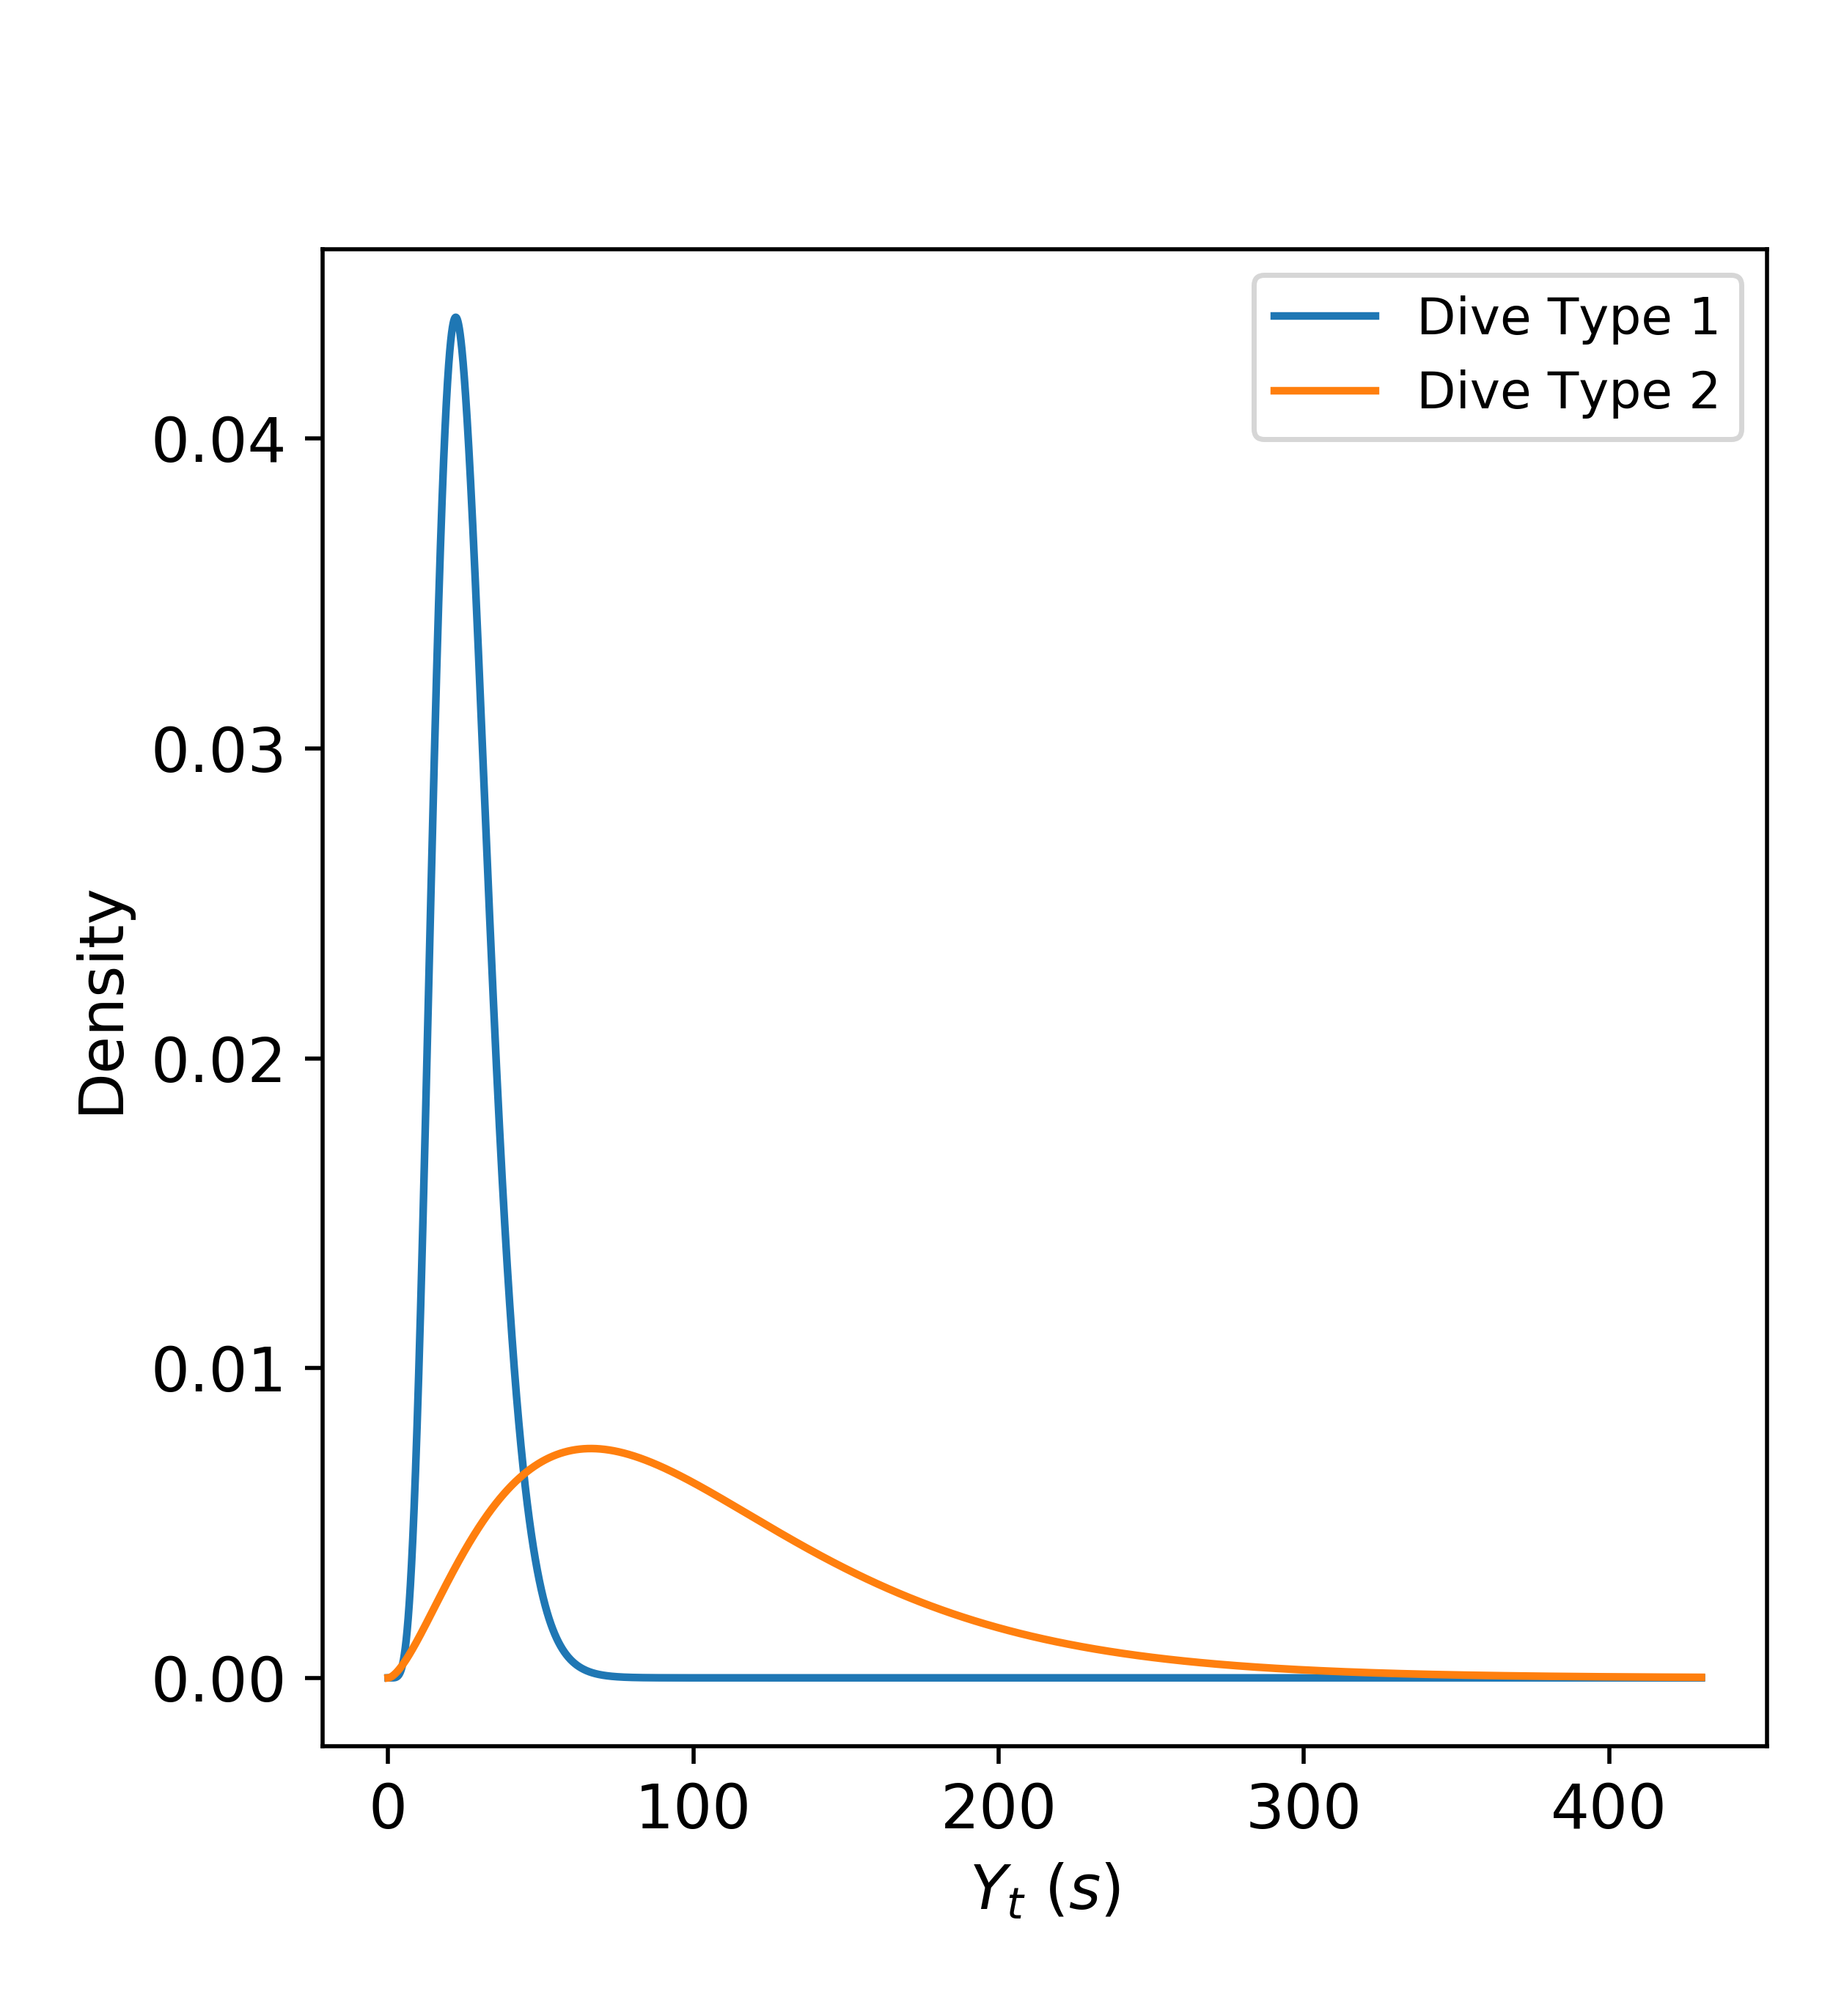
\includegraphics[width=5in]{../Plots/CarHHMM2-coarse-emissions.png}
	\caption{Estimated probability distributions for each coarse-scale observation in each dive type.}
	\label{fig:coarse_emis}
\end{figure}

\begin{figure}[ht]
	\centering
	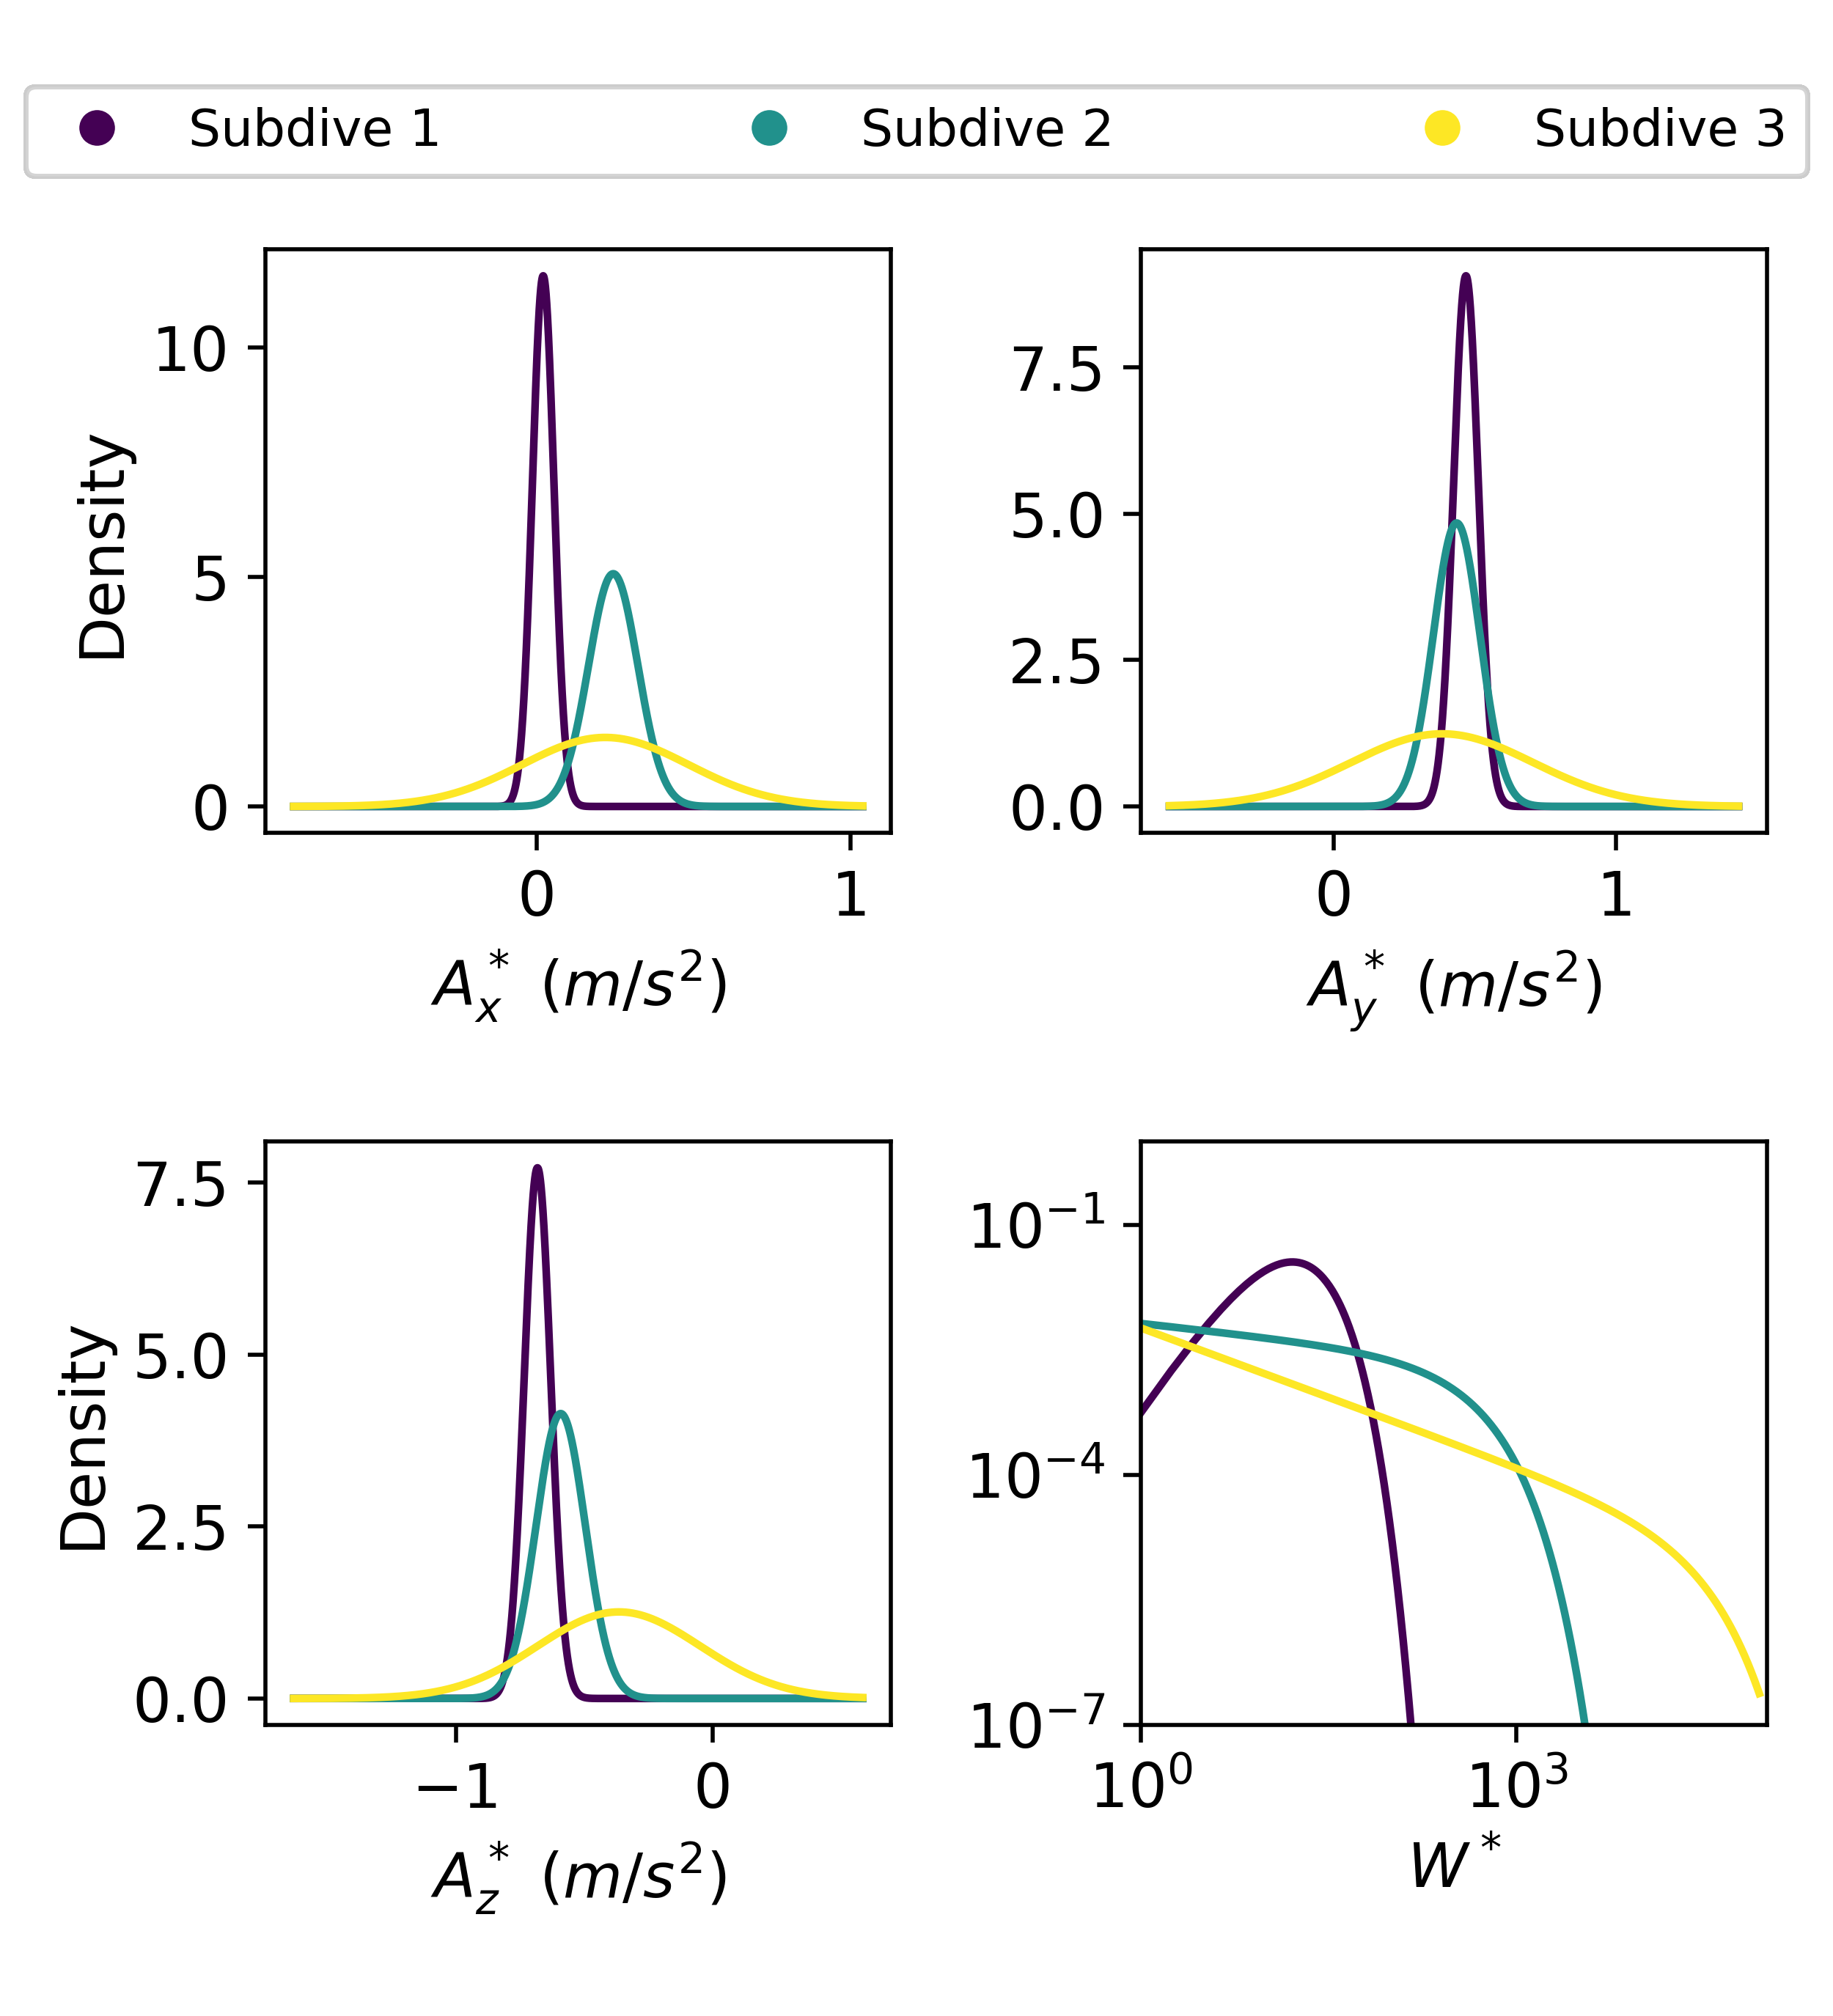
\includegraphics[width=5in]{../Plots/CarHHMM2-fine-emissions.png}
	\caption{Estimated probability distributions for each fine-scale observation in each behavioral state. Note that the distributions of acceleration do not take auto-correlation into account (see table \ref{table:emis_dists})}
	\label{fig:fine_emis}
\end{figure}

\begin{figure}[ht]
	\centering
	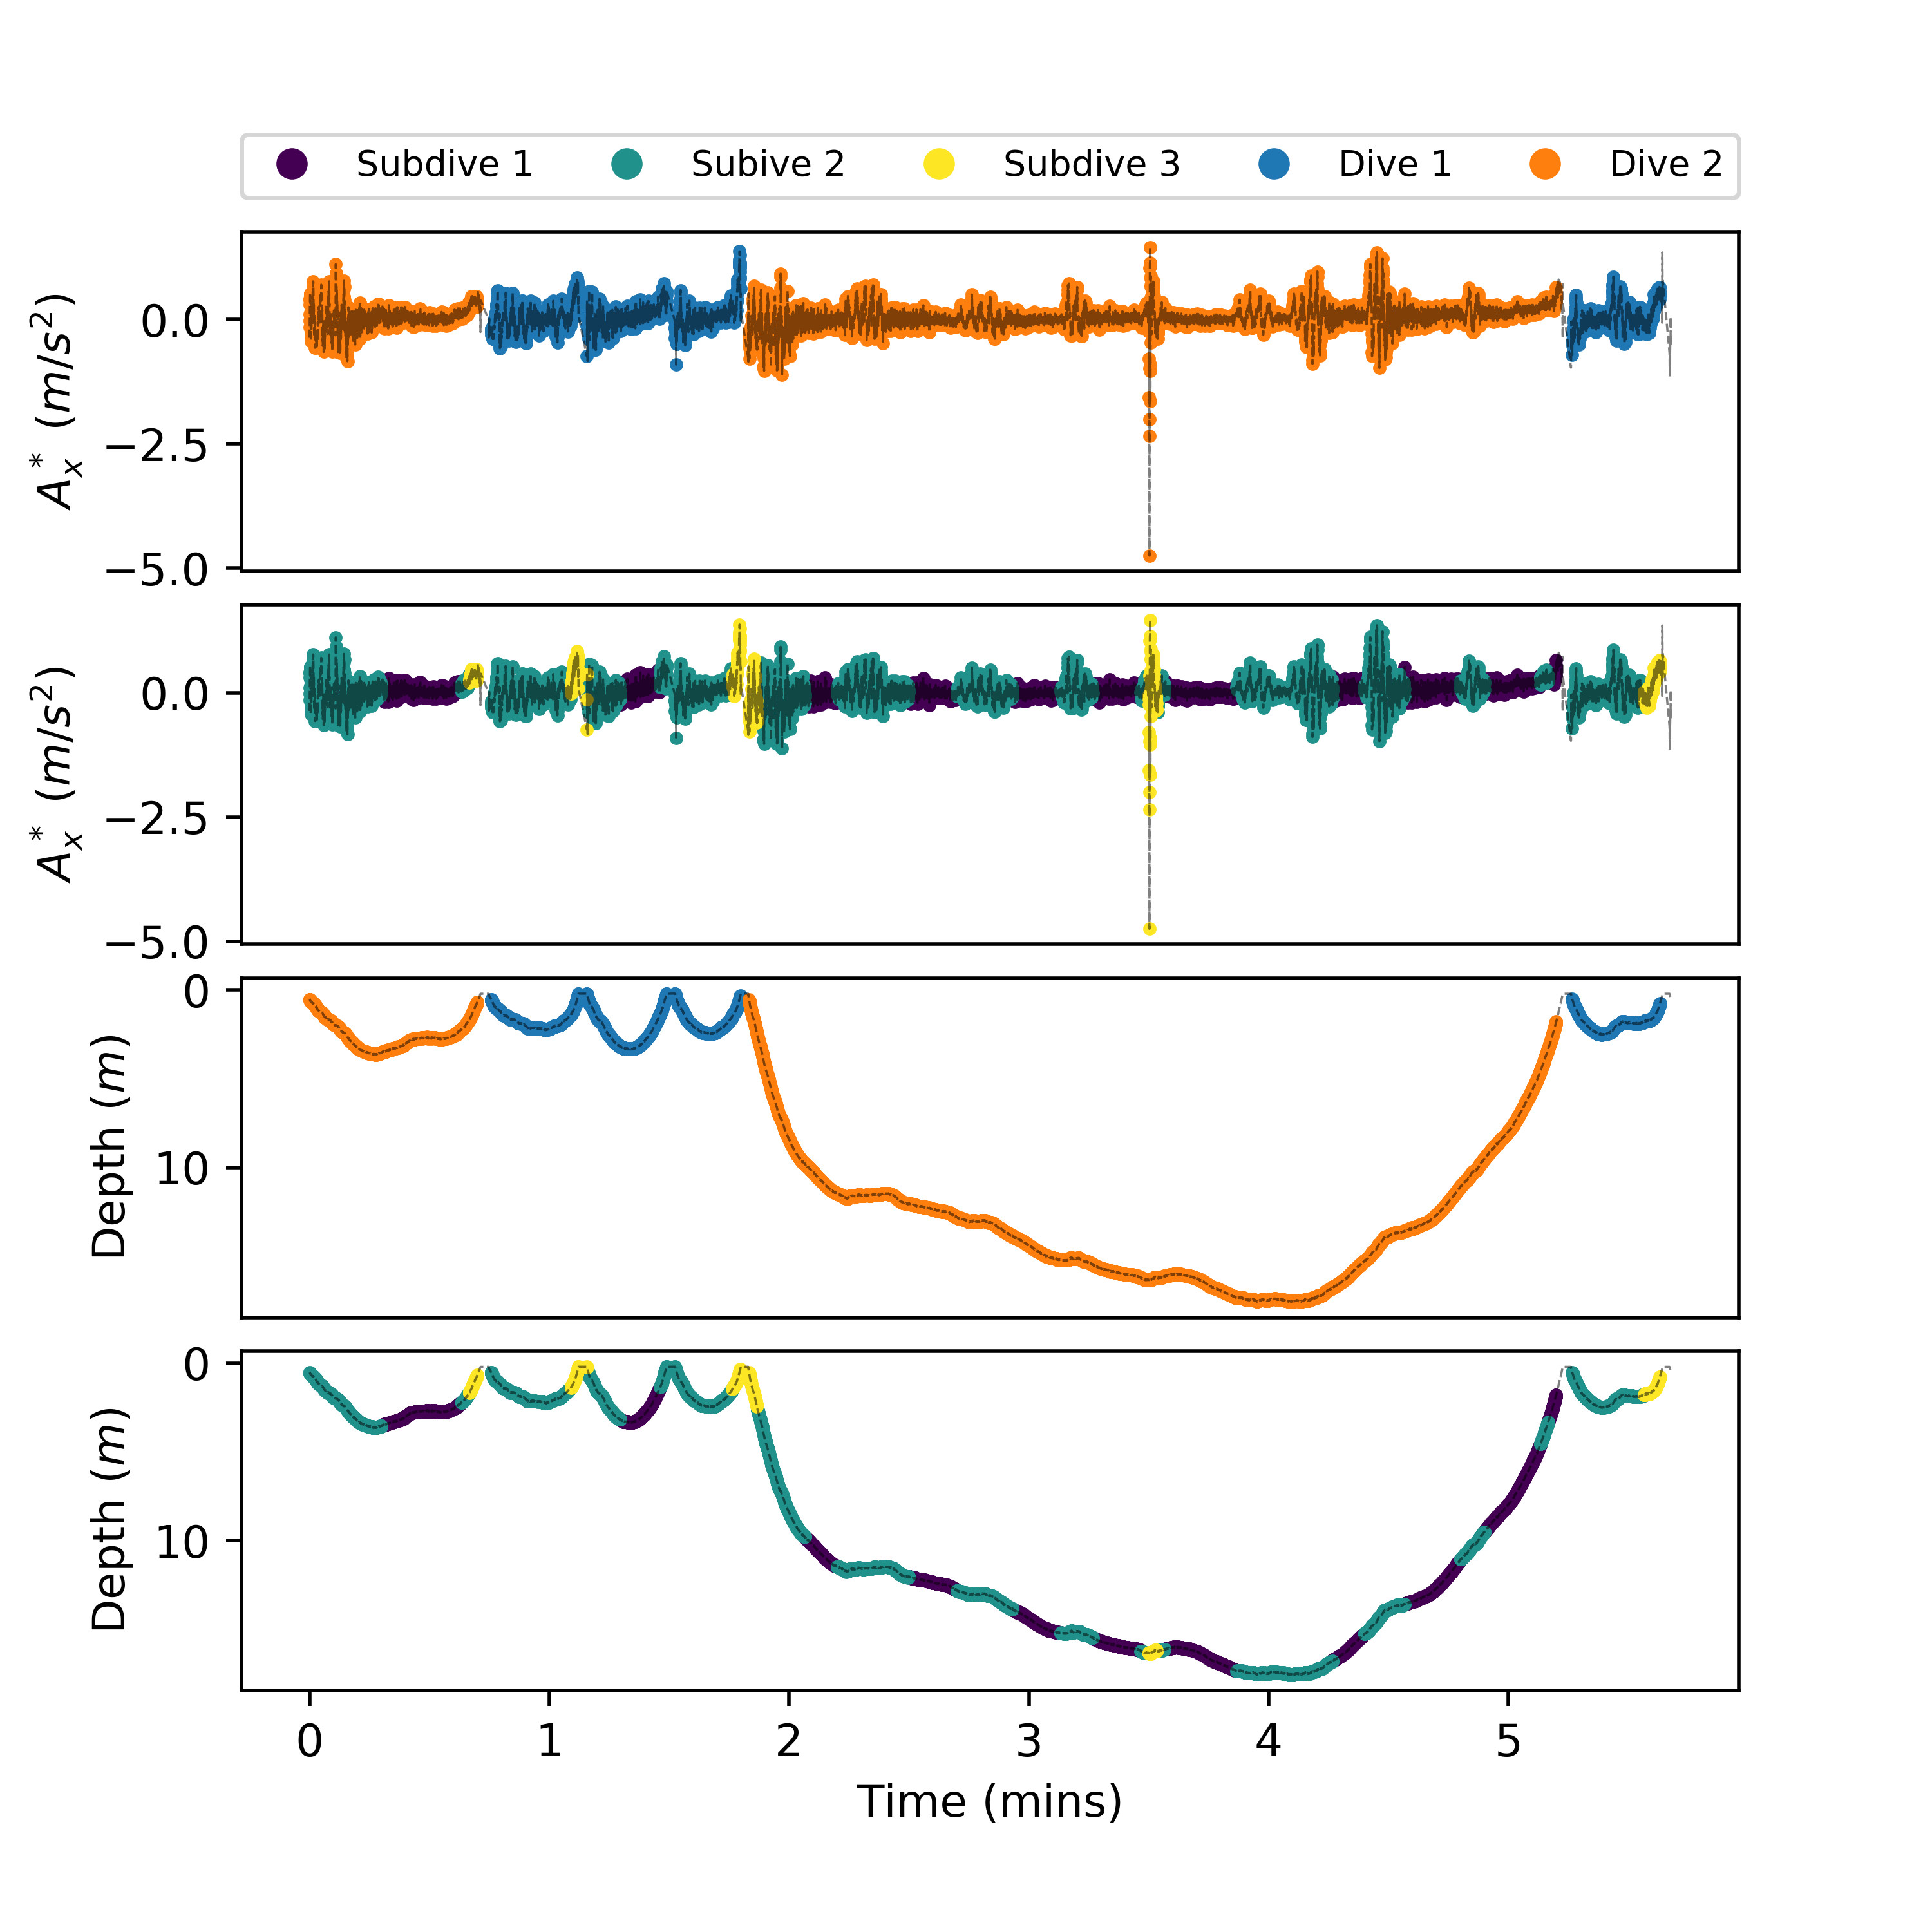
\includegraphics[width=5in]{../Plots/CarHHMM2_decoded_dives.png}
	\caption{Features of a particular set of killer whale dives and decoded estimates for the intra-dive behavioral states. The color of the plot corresponds to behavioral or dive state with the highest probability.}
	\label{fig:labeled_dives}
\end{figure}

\begin{figure}[ht]
    \begin{subfigure}{0.45\textwidth}
    	\centering
    	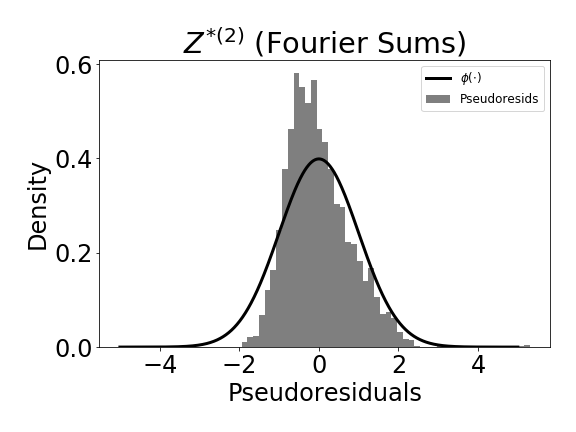
\includegraphics[width=2.25in]{../Plots/CarHHMM2_psedoresids_ahat.png}
    	\caption{Pseudoresiduals of $Z^{*(2)}$}
    	\label{fig:pseudoresids}
    \end{subfigure}
    \begin{subfigure}{0.45\textwidth}
    	\centering
    	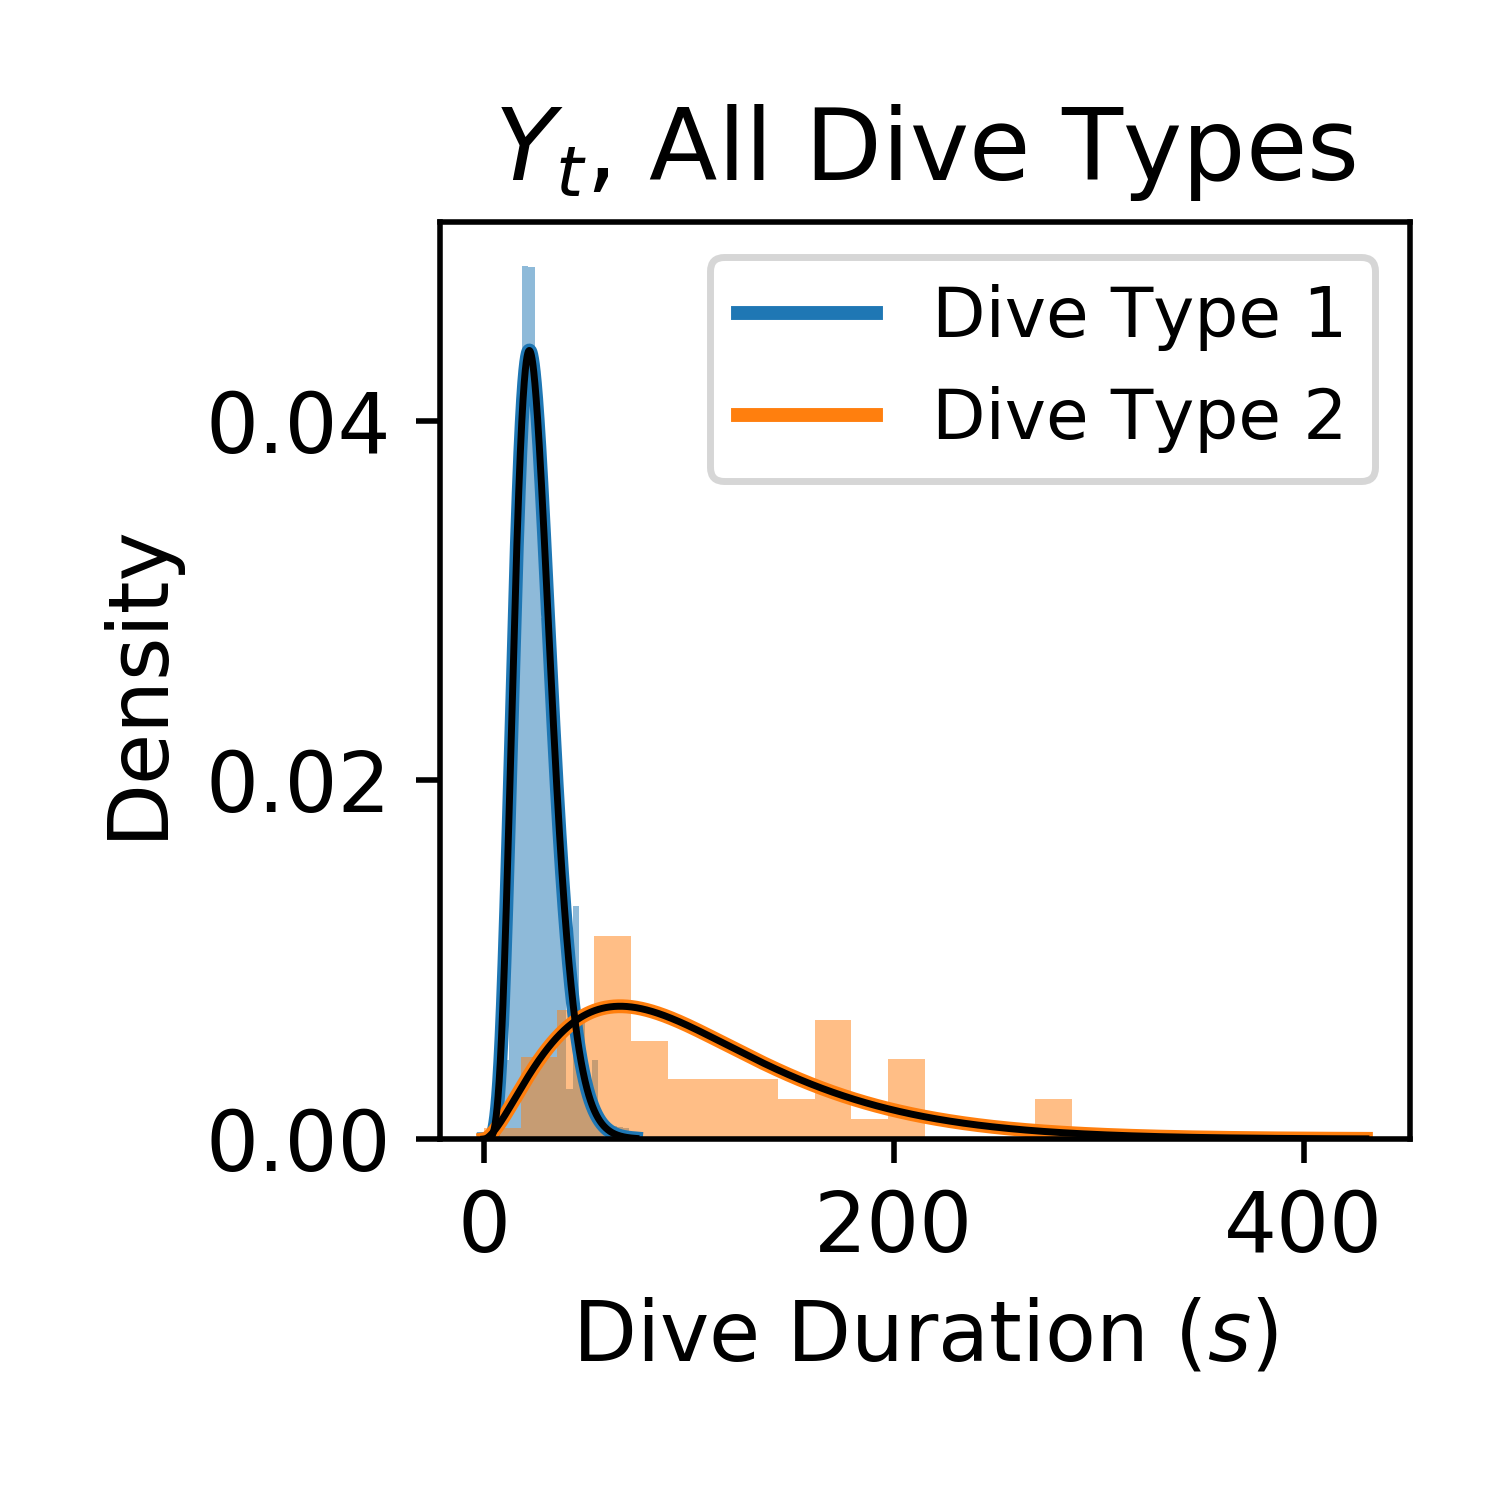
\includegraphics[width=2.25in]{../Plots/CarHHMM2_empirical_hist_dive_duration.png}
    	\caption{Empirical distribution of $Y$ (Dive Duration)}
    	\label{fig:empirical_dist}
    \end{subfigure}
    \caption{Examples of psuedoresiduals and a weighted empirical distribution as model checking tools}
    \label{fig:model_checking}
\end{figure}